% !TEX program = xelatex
\documentclass[a4paper]{exam}
\usepackage{amsmath}
\usepackage{amsthm}
\usepackage[left=1.8cm,right=1.8cm,top=2.2cm,bottom=2.0cm]{geometry}
\usepackage[UTF8]{ctex}
\usepackage{enumerate}
\usepackage{fancyhdr}
\usepackage{xpatch}
\usepackage{graphicx} 
\usepackage{float} 
\usepackage{subfigure} 
\usepackage{amsfonts}
\usepackage{mathtools}
\usepackage{framed}
\usepackage{multicol}
\usepackage{hyperref}
\usepackage{fontspec}
\usepackage{float}
\usepackage{tikz}
\usepackage{alltt}
\usepackage{multicol,comment}
\usepackage{biblatex}
\addbibresource{02-discussion.bib}
\usetikzlibrary{automata,positioning}
\usepackage[section]{placeins}
\makeatletter

\printanswers


\AtBeginDocument{\xpatchcmd{\@thm}{\thm@headpunct{.}}{\thm@headpunct{}}{}{}}
\makeatother

\pagestyle{fancy}
\renewcommand{\baselinestretch}{1.15}
\newcommand{\code}[1]{\texttt{#1}}
\usepackage{paralist}
\let\itemize\compactitem
\let\enditemize\endcompactitem
\let\enumerate\compactenum
\let\endenumerate\endcompactenum
\let\description\compactdesc
\let\enddescription\endcompactdesc

% shorten footnote rule
\xpatchcmd\footnoterule
  {.4\columnwidth}
  {1in}
  {}{\fail}

\title{CS 131 Compilers: Discussion 3: LL and LR Parsers}
\author{\textbf{杨易为}~~\textbf{吴凌云}~~\textbf{樊雨鑫} \\ \texttt{ \{yangyw,wuly2,fanyx\}@shanghaitech.edu.cn}}

\begin{document}
\maketitle
% \section{DFA and NFA}
% \subsection{Introduction}
\section{LL Parsing Ambiguities}
 An LL(k) grammar is a CFG used by a parser that scans
input left-to-right (“L”), leftmost derivation (“L”), and uses k tokens of lookahead to
predict the correct production. We’ve previously seen that a grammar is ambiguous
if it has a parse tree that is not unique. A more formal definition of LL conflicts uses
FIRST and FOLLOW sets.

\begin{enumerate}
  \item \textbf{FIRST(A)}  the set of all terminals that could occur first in an expansion of
  the terminal or nonterminal A (include $\epsilon$ if A can expand to $\epsilon$)
  \item \textbf{FOLLOW(A)}  the set of all terminals that could follow an occurrence of the
  terminal or nonterminal A in a (partial) derivation.
\end{enumerate}

\subsection{There are two main types of LL(1) conflicts:}
\begin{enumerate}
  \item \textbf{FIRST/FIRST} The FIRST sets of two different productions for same nonterminal intersect.
  \item \textbf{FIRST/FOLLOW}: The FIRST set of a grammar rule contains an epsilon and
  the intersection with its FOLLOW set is not empty.

\end{enumerate}

Is the following grammar LL(1)? Justify your answer using FIRST and FOLLOW sets.

$$S → Xd$$
$$X → C | Ba$$
$$C →\epsilon $$
$$B → d$$

\begin{solution}
This is an instance of a FIRST/FOLLOW conflict. FIRST(X) contains the empty string and the intersection of $\operatorname{FIRST}(\mathrm{X})$ and $\operatorname{FOLLOW}(\mathrm{X})$ is not empty:
$\operatorname{FIRST}(\mathrm{S})=\operatorname{FIRST}(\mathrm{x} \mathrm{d})=\left\{\mathrm{d}^{\prime}\right\} \quad \mathrm{FIRST}(\mathrm{x})=\operatorname{FIRST}(\mathrm{C}) \cup \operatorname{FIRST}(\mathrm{B}$ a) $\quad \operatorname{FIRST}(\mathrm{C})=\{\epsilon\}$
$$
\operatorname{FIRST}(\mathrm{B} a)=\left\{{ }^{\prime} \mathrm{d}^{\prime}\right\} \quad \operatorname{FIRST}(\mathrm{B})=\left\{\mathrm{d}^{\prime}\right\}
$$
FOLLOW $(\mathrm{S})=\{\} \quad \operatorname{FOLLOW}(\mathrm{x})=\left\{\mathrm{d}^{\prime}\right\} \quad \operatorname{FOLLOW}(\mathrm{C})=\left\{\mathrm{d}^{\prime}\right\} \quad$ FOLLOW $(\mathrm{B})=\left\{\right.$ 'a $\left.^{\prime}\right\}$
\end{solution}


\section{Resolving Conflicts}
Consider the following grammar for numerical expressions with division, addition, and
unary minus:

$$\text{ E } → \text{ Num } |\text{ E / E } | \text{ E + E } | \text{ − E}$$

\begin{enumerate}
  \item Rewrite the grammar so that it is LL(1), so that ‘/’ has higher precedence than
  ‘+’, and so that ‘-’ has highest precedence. ‘+’ and ‘/’ should be parsed in a
  right-associative way.
  \item  Compute the FIRST and FOLLOW sets for your re-written LL(1) grammar.
  \item Draw the LL(1) parsing table for the grammar. You may need the following rules:
  \begin{enumerate}
    \item  For each production $X \rightarrow A_{1} \ldots A_{n}:$
    \item For each $1 \leq i \leq n,$ and for each $b$ in First $\left(A_{i}\right):$ Set $T[X, b]=X \rightarrow$
    $A_{1} \ldots A_{n} .$ Stop when $\epsilon$ is not in First $\left(A_{i}\right) .$
    \item If $A_{1} \ldots A_{n} \rightarrow^{*} \epsilon,$ then for each $b$ in Follow $(X):$ Set $T[X, b]=\epsilon$
  \end{enumerate}
\end{enumerate}
\begin{solution}
\begin{enumerate}
    \item \begin{multicols}{3}
        \begin{alltt}
        expr : expr1 rest
        
        rest : \(\epsilon\)
             | '+' expr
        
        expr1 : expr2 rest1
        
        rest1 : \(\epsilon\)
              | '/' expr1
        
        expr2 : '-' expr2
              | NUM
        \end{alltt}
    \end{multicols}
    \item FIRST $(\operatorname{expr} 1$ rest $)=$ FIRST $($ expr2 rest1 $)=\left\{-\right.$, NUM $\}$
    \\
    
    FIRST(’+’ expr) = { ’+’ }\\
    FIRST(’-’ expr2) = { ’-’ }\\
    FIRST($\epsilon$) = { $\epsilon$ }\\
    FIRST(’/’ expr1) = { ’/’ }\\
    FIRST(NUM) = { NUM }\\
    
\\
FOLLOW $(\operatorname{expr} 2)=\{ '/', '+', \dashv \}$\\
FOLLOW $($ expr 1$)=$ FOLLOW $($ rest1 $)=\left\{{ }^{\prime}+{ }^{\prime}, \dashv\right\}$\\
FOLLOW $($ expr $)=$ FOLLOW $($ rest $)=\{\dashv\}$\\
\item \begin{tabular}{|c|ccccc|}
\hline & $-$ & $N U M$ & $/$ & $+$ & $-$ \\
expr & expr $\rightarrow$ expr1rest & expr $\rightarrow$ expr1rest & & & \\
rest & & & & rest $\rightarrow+$ expr & $\epsilon$ \\
expr1 & expr1 $\rightarrow$ expr2rest1 & expr1 $\rightarrow$ expr2rest1 & & & \\
rest1 & & & rest1 $\rightarrow /$ expr 1 & $\epsilon$ & $\epsilon$ \\
expr2 & expr2 $\rightarrow-$ expr2 & expr2 $\rightarrow$ NUM & & & $\epsilon$ \\
\hline
\end{tabular}
\end{enumerate}
\end{solution}

\section{Earley's Algorithm}
Consider the following CFG with terminals $\{(,),+, *, a, b\}$ (+ represents union) that is
used to represent regular expressions over alphabet $\{a, b\}$ :

$$P \rightarrow E \dashv$$
$$E \rightarrow E+E$$
$$E \rightarrow E * E$$
$$E \rightarrow I D$$
\begin{enumerate}
  \item Using the above CFG, use Earley's Algorithm for the following input string $I D+I D * I D$.
  \item For the derivation in above solution, provide the corresponding parse tree.
\end{enumerate}
\begin{figure}[htbp]
    \centering
    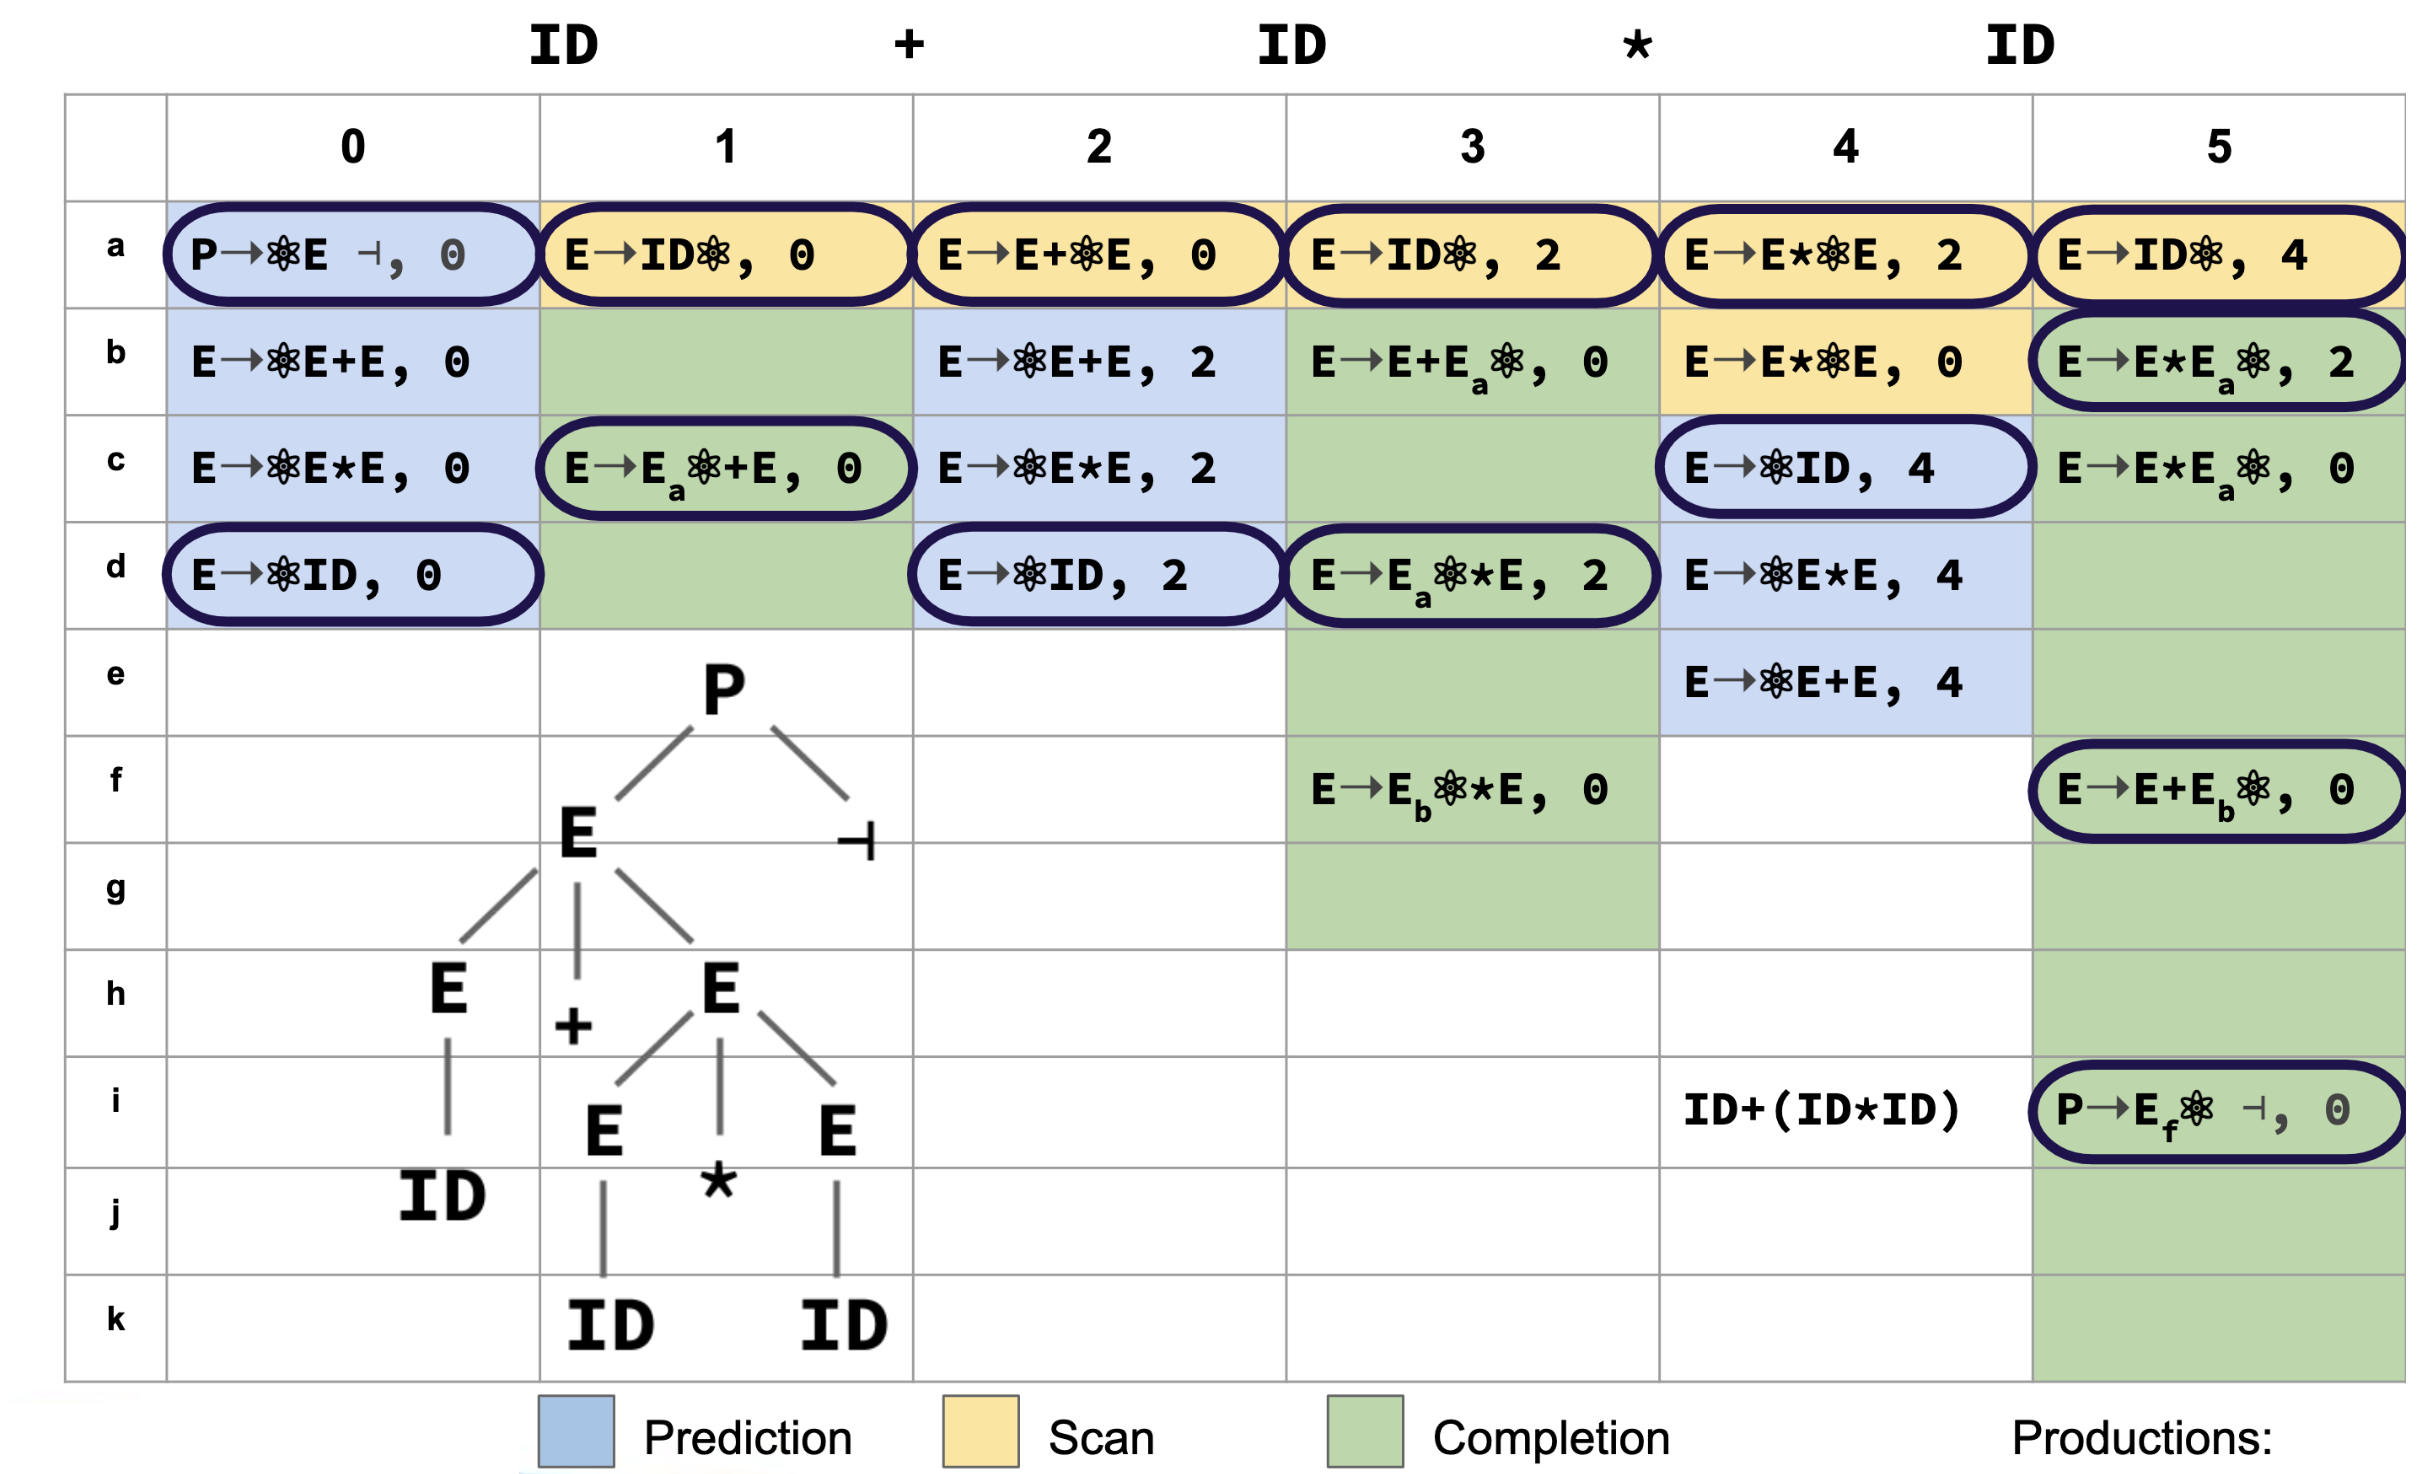
\includegraphics[width=\columnwidth]{./img/first.png}
  \end{figure}
  
  \begin{figure}[htbp]
    \centering
    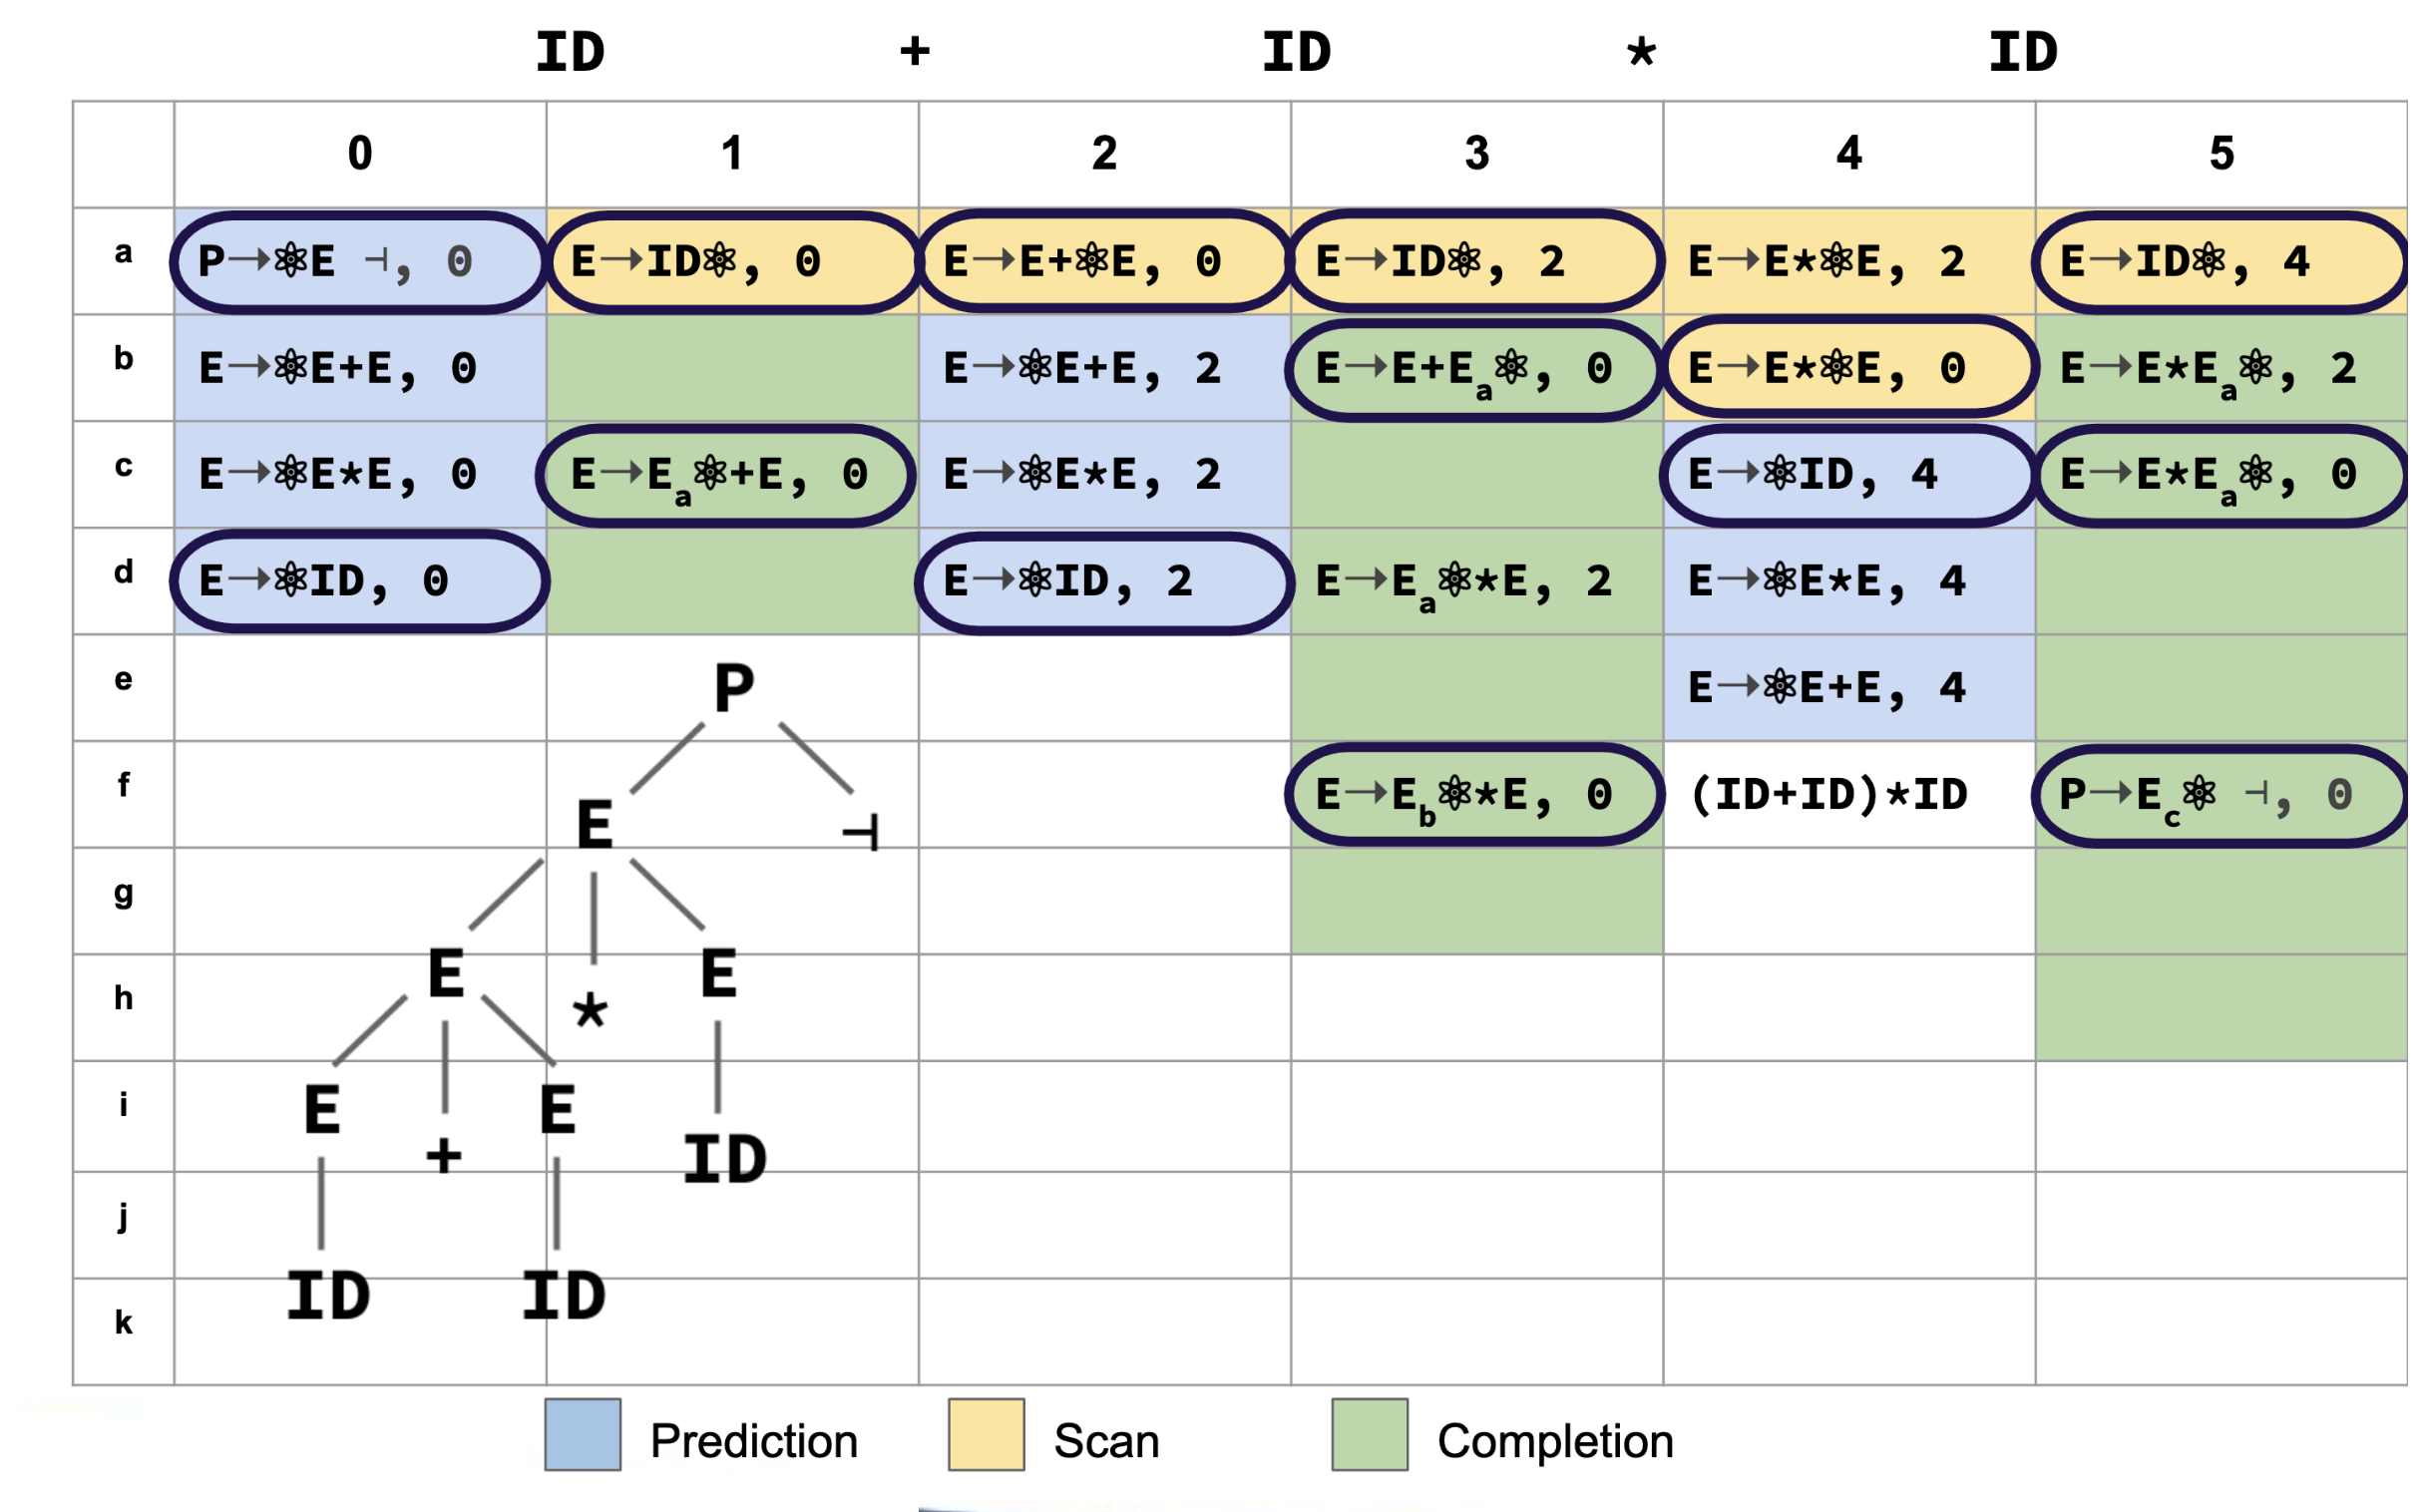
\includegraphics[width=\columnwidth]{./img/second.png}
  \end{figure}
\begin{solution}



\end{solution}

\section{LR(k) automata}
The procedure of shifting the next Token and reducing at certain points is exactly like going through an Automata. Therefore we can build a $L R(0)$ Automata to do the Bottom-Up Parsing.

A Handle is a pair $(r, p)$, where $r$ is a Production Rule $A \rightarrow s$, and $p$ is the position of $s$ when $r$ is used in the Derivation step. Unambiguous Grammar has exactly one set of handles for a Right-most Derivation.

A Viable Prefix is a sequence that can be the stack content, which CANNOT extend past the right end of a Handle. Production Rule $A \rightarrow \beta_{1} \beta_{2}$ is Valid for Viable Prefix $\alpha \beta_{1}$ iff $S \Rightarrow^{*} \alpha A \gamma \Rightarrow \alpha \beta_{1} \beta_{2} \gamma$
\begin{enumerate}
    \item If $\beta_{2}=\varepsilon$, should Reduce
    \item If $\beta_{2} \neq \varepsilon$, should Shift
\end{enumerate}
An $L R(0)$ Item $A \rightarrow \beta_{1} \cdot \beta_{2}$ means that:
\begin{enumerate}
    \item Production Rule $A \rightarrow \beta_{1} \beta_{2}$ is Valid for current Viable Prefix
\item We have shifted things in $\beta_{1}$ onto stack, but things in $\beta_{2}$ not met yet 
\item No information about next Tokens, i.e. no Look-aheads
\end{enumerate}

\subsection{Consider the following two grammars $G_1$ and $G_2$, where one of them is an ambiguous grammar and the another one is a non-ambiguous grammar.}
\begin{multicols}{2}
$\\G_1$, $S$ is the start symbol\\
$S$ \rightarrow a B S \mid b A S \\
S \rightarrow \varepsilon \\
A \rightarrow a \mid b A A \\
B \rightarrow b \mid \text { a B } B\\
$G_2$, $S$ is the start symbol\\
$S$ \rightarrow a B \mid b A \\
S \rightarrow \varepsilon \\
A \rightarrow a S \mid b A A \\
B \rightarrow b S \mid a B B
\end{multicols}
\begin{parts}
\part[5] Which grammar is ambiguous? Use $aababb$ to prove its ambiguity.
\begin{solution}
$G_2$ is ambiguous, because it has 2 left most deriviation.\\
$S=>_{lm} aB=>_{lm} aaBB=>_{lm}aabSB =>_{lm} aabB =>_{lm} aabaBB =>_{lm}$\\
$aababSB=>_{lm}aababB=>_{lm}aababbS=>_{lm}aababb$\\

$S=>_{lm}aB=>_{lm}aaBB=>_{lm}aabSB=>_{lm}aabaBB=>_{lm}aababSB=>_{lm}$\\
$aababB=>_{lm}aababbS=>_{lm}aababb$

\end{solution}



\part[10] For the non-ambiguous grammar, write down the fragment of the LR(0) automaton such that
this fragment accepts the input word 
 $aBaaBB$. Here fragment means some states and some transitions between states of the LR(0) automaton.
\begin{solution}
$G_1$ is non-ambiguous.\\
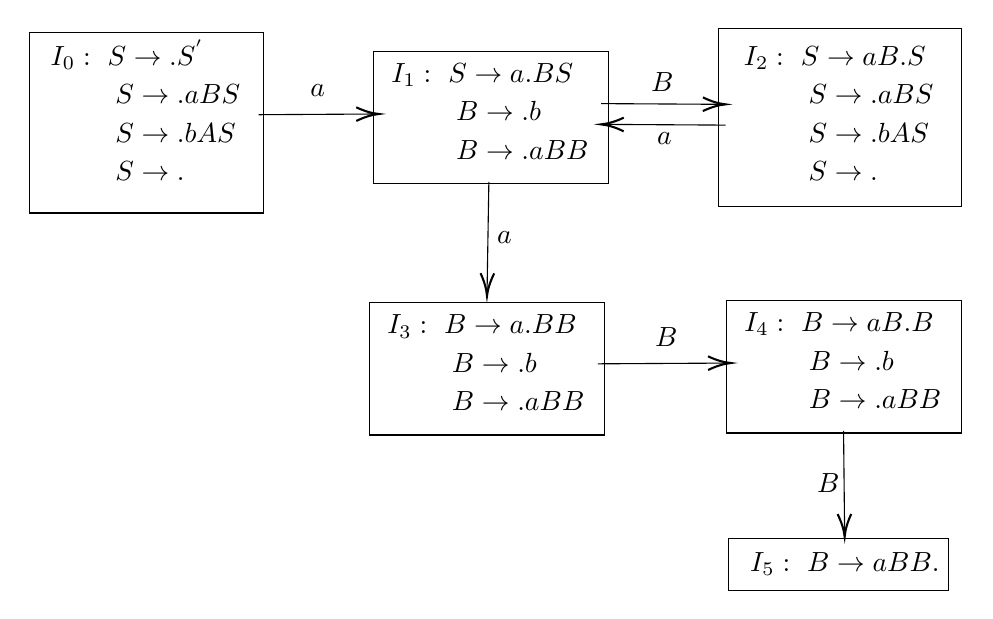
\begin{tikzpicture}[x=0.75pt,y=0.75pt,yscale=-1,xscale=1]
%uncomment if require: \path (0,361); %set diagram left start at 0, and has height of 361

%Shape: Rectangle [id:dp04467084256653531] 
\draw   (14,18) -- (127,18) -- (127,105) -- (14,105) -- cycle ;
%Shape: Rectangle [id:dp38216533659480145] 
\draw   (180,27) -- (293,27) -- (293,91) -- (180,91) -- cycle ;
%Shape: Rectangle [id:dp6729083597465751] 
\draw   (346,16) -- (463,16) -- (463,102) -- (346,102) -- cycle ;
%Shape: Rectangle [id:dp5855748639899848] 
\draw   (178,148) -- (291,148) -- (291,212) -- (178,212) -- cycle ;
%Shape: Rectangle [id:dp39750860053051695] 
\draw   (350,147) -- (463,147) -- (463,211) -- (350,211) -- cycle ;
%Shape: Rectangle [id:dp6637178303801441] 
\draw   (351,262) -- (457,262) -- (457,287) -- (351,287) -- cycle ;

% Text Node
\draw (70,58) node    {$ \begin{array}{l}
I_{0} :\ S\rightarrow .S^{'}\\
\ \ \ \ \ \ \ S\rightarrow .aBS\\
\ \ \ \ \ \ \ S\rightarrow .bAS\\
\ \ \ \ \ \ \ S\rightarrow .
\end{array}$};
% Text Node
\draw (236,57) node    {$ \begin{array}{l}
I_{1} :\ S\rightarrow a.BS\\
\ \ \ \ \ \ \ B\rightarrow .b\\
\ \ \ \ \ \ \ B\rightarrow .aBB
\end{array}$};
% Text Node
\draw (404,58) node    {$ \begin{array}{l}
I_{2} :\ S\rightarrow aB.S\\
\ \ \ \ \ \ \ S\rightarrow .aBS\\
\ \ \ \ \ \ \ S\rightarrow .bAS\\
\ \ \ \ \ \ \ S\rightarrow .
\end{array}$};
% Text Node
\draw (234,178) node    {$ \begin{array}{l}
I_{3} :\ B\rightarrow a.BB\\
\ \ \ \ \ \ \ B\rightarrow .b\\
\ \ \ \ \ \ \ B\rightarrow .aBB
\end{array}$};
% Text Node
\draw (406,177) node    {$ \begin{array}{l}
I_{4} :\ B\rightarrow aB.B\\
\ \ \ \ \ \ \ B\rightarrow .b\\
\ \ \ \ \ \ \ B\rightarrow .aBB
\end{array}$};
% Text Node
\draw (407,274) node    {$I_{5} :\ B\rightarrow aBB.$};
% Text Node
\draw (153,46) node    {$a$};
% Text Node
\draw (319,42) node    {$B$};
% Text Node
\draw (320,69) node    {$a$};
% Text Node
\draw (243,117) node    {$a$};
% Text Node
\draw (321,165) node    {$B$};
% Text Node
\draw (399,235) node    {$B$};
% Connection
\draw    (124.5,57.67) -- (180.5,57.33) ;
\draw [shift={(182.5,57.32)}, rotate = 539.65] [color={rgb, 255:red, 0; green, 0; blue, 0 }  ][line width=0.75]    (10.93,-3.29) .. controls (6.95,-1.4) and (3.31,-0.3) .. (0,0) .. controls (3.31,0.3) and (6.95,1.4) .. (10.93,3.29)   ;
% Connection
\draw    (289.5,52.32) -- (347.5,52.66) ;
\draw [shift={(349.5,52.68)}, rotate = 180.34] [color={rgb, 255:red, 0; green, 0; blue, 0 }  ][line width=0.75]    (10.93,-3.29) .. controls (6.95,-1.4) and (3.31,-0.3) .. (0,0) .. controls (3.31,0.3) and (6.95,1.4) .. (10.93,3.29)   ;
% Connection
\draw    (349.5,62.68) -- (291.5,62.33) ;
\draw [shift={(289.5,62.32)}, rotate = 360.34000000000003] [color={rgb, 255:red, 0; green, 0; blue, 0 }  ][line width=0.75]    (10.93,-3.29) .. controls (6.95,-1.4) and (3.31,-0.3) .. (0,0) .. controls (3.31,0.3) and (6.95,1.4) .. (10.93,3.29)   ;
% Connection
\draw    (235.45,90) -- (234.58,143) ;
\draw [shift={(234.55,145)}, rotate = 270.95] [color={rgb, 255:red, 0; green, 0; blue, 0 }  ][line width=0.75]    (10.93,-3.29) .. controls (6.95,-1.4) and (3.31,-0.3) .. (0,0) .. controls (3.31,0.3) and (6.95,1.4) .. (10.93,3.29)   ;
% Connection
\draw    (288,177.69) -- (350,177.33) ;
\draw [shift={(352,177.31)}, rotate = 539.6700000000001] [color={rgb, 255:red, 0; green, 0; blue, 0 }  ][line width=0.75]    (10.93,-3.29) .. controls (6.95,-1.4) and (3.31,-0.3) .. (0,0) .. controls (3.31,0.3) and (6.95,1.4) .. (10.93,3.29)   ;
% Connection
\draw    (406.34,210) -- (406.85,259) ;
\draw [shift={(406.87,261)}, rotate = 269.40999999999997] [color={rgb, 255:red, 0; green, 0; blue, 0 }  ][line width=0.75]    (10.93,-3.29) .. controls (6.95,-1.4) and (3.31,-0.3) .. (0,0) .. controls (3.31,0.3) and (6.95,1.4) .. (10.93,3.29)   ;

\end{tikzpicture}

\end{solution}

\part[15] For the non-ambiguous grammar, write down the fragment of the LR(1) automaton such that this fragment accepts the input word $aBaaaB$. Here fragment means some states and some transitions between states of the LR(1) automaton.
\begin{solution}
\\
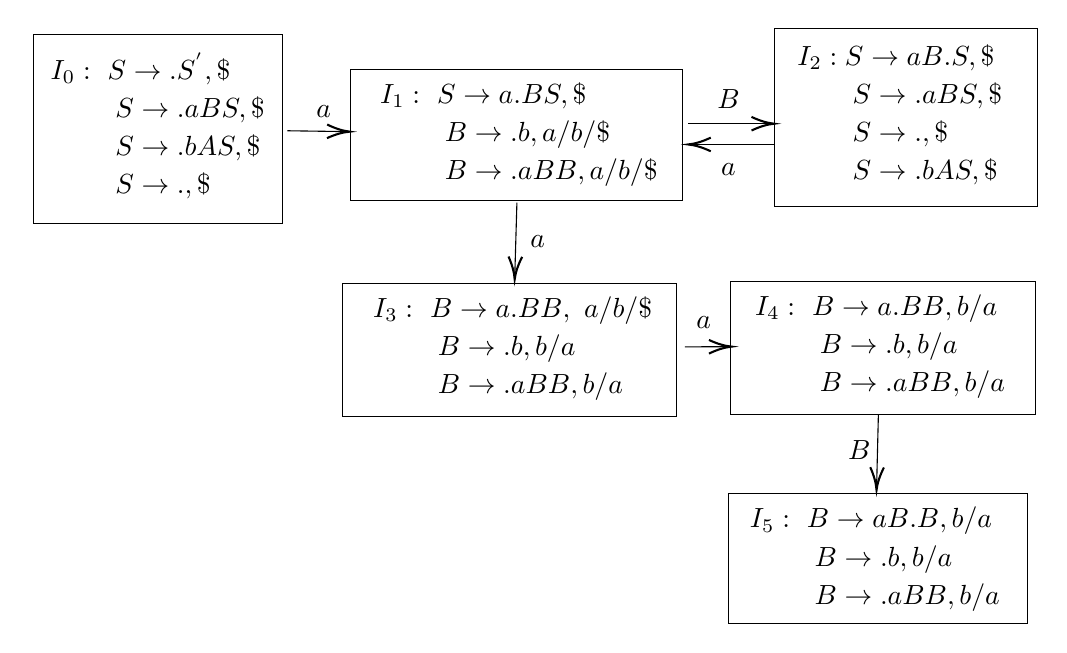
\begin{tikzpicture}[x=0.75pt,y=0.75pt,yscale=-1,xscale=1]
%uncomment if require: \path (0,361); %set diagram left start at 0, and has height of 361

%Shape: Rectangle [id:dp21193032753981977] 
\draw   (34,48) -- (154,48) -- (154,139) -- (34,139) -- cycle ;
%Shape: Rectangle [id:dp057585357617519595] 
\draw   (187,65) -- (347,65) -- (347,128) -- (187,128) -- cycle ;
%Shape: Rectangle [id:dp4993922983958634] 
\draw   (391,45) -- (518,45) -- (518,131) -- (391,131) -- cycle ;
%Shape: Rectangle [id:dp6480767825445916] 
\draw   (183,168) -- (344,168) -- (344,232) -- (183,232) -- cycle ;
%Shape: Rectangle [id:dp8888242275807938] 
\draw   (370,167) -- (517,167) -- (517,231) -- (370,231) -- cycle ;
%Shape: Rectangle [id:dp13659478006442416] 
\draw   (369,269) -- (513,269) -- (513,332) -- (369,332) -- cycle ;

% Text Node
\draw (94,93.5) node    {$ \begin{array}{l}
I_{0} :\ S\rightarrow .S^{'} ,\$\\
\ \ \ \ \ \ \ S\rightarrow .aBS,\$\\
\ \ \ \ \ \ \ S\rightarrow .bAS,\$\\
\ \ \ \ \ \ \ S\rightarrow .,\$
\end{array}$};
% Text Node
\draw (268,96) node    {$ \begin{array}{l}
I_{1} :\ S\rightarrow a.BS,\$\\
\ \ \ \ \ \ \ B\rightarrow .b,a/b/\$\\
\ \ \ \ \ \ \ B\rightarrow .aBB,a/b/\$
\end{array}$};
% Text Node
\draw (451.5,96) node    {$ \begin{array}{l}
I_{2} :S\rightarrow aB.S,\$\\
\ \ \ \ \ \ S\rightarrow .aBS,\$\\
\ \ \ \ \ \ S\rightarrow .,\$\\
\ \ \ \ \ \ S\rightarrow .bAS,\$\\
\ \ \ \ \ 
\end{array}$};
% Text Node
\draw (265,199) node    {$ \begin{array}{l}
I_{3} :\ B\rightarrow a.BB,\ a/b/\$\\
\ \ \ \ \ \ \ B\rightarrow .b,b/a\\
\ \ \ \ \ \ \ B\rightarrow .aBB,b/a
\end{array}$};
% Text Node
\draw (442,198) node    {$ \begin{array}{l}
I_{4} :\ B\rightarrow a.BB,b/a\\
\ \ \ \ \ \ \ B\rightarrow .b,b/a\\
\ \ \ \ \ \ \ B\rightarrow .aBB,b/a
\end{array}$};
% Text Node
\draw (439.5,300.5) node    {$ \begin{array}{l}
I_{5} :\ B\rightarrow aB.B,b/a\\
\ \ \ \ \ \ \ B\rightarrow .b,b/a\\
\ \ \ \ \ \ \ B\rightarrow .aBB,b/a
\end{array}$};
% Text Node
\draw (174,85) node    {$a$};
% Text Node
\draw (369,79) node    {$B$};
% Text Node
\draw (357,187) node    {$a$};
% Text Node
\draw (432,248) node    {$B$};
% Text Node
\draw (369,113) node    {$a$};
% Text Node
\draw (277,148) node    {$a$};
% Connection
\draw    (156.5,94.4) -- (184.5,94.8) ;
\draw [shift={(186.5,94.83)}, rotate = 180.82] [color={rgb, 255:red, 0; green, 0; blue, 0 }  ][line width=0.75]    (10.93,-3.29) .. controls (6.95,-1.4) and (3.31,-0.3) .. (0,0) .. controls (3.31,0.3) and (6.95,1.4) .. (10.93,3.29)   ;
% Connection
\draw    (349.5,91) -- (389,91) ;
\draw [shift={(391,91)}, rotate = 180] [color={rgb, 255:red, 0; green, 0; blue, 0 }  ][line width=0.75]    (10.93,-3.29) .. controls (6.95,-1.4) and (3.31,-0.3) .. (0,0) .. controls (3.31,0.3) and (6.95,1.4) .. (10.93,3.29)   ;
% Connection
\draw    (267.04,129) -- (266.02,164) ;
\draw [shift={(265.96,166)}, rotate = 271.67] [color={rgb, 255:red, 0; green, 0; blue, 0 }  ][line width=0.75]    (10.93,-3.29) .. controls (6.95,-1.4) and (3.31,-0.3) .. (0,0) .. controls (3.31,0.3) and (6.95,1.4) .. (10.93,3.29)   ;
% Connection
\draw    (348,198.53) -- (368.5,198.42) ;
\draw [shift={(370.5,198.4)}, rotate = 539.6800000000001] [color={rgb, 255:red, 0; green, 0; blue, 0 }  ][line width=0.75]    (10.93,-3.29) .. controls (6.95,-1.4) and (3.31,-0.3) .. (0,0) .. controls (3.31,0.3) and (6.95,1.4) .. (10.93,3.29)   ;
% Connection
\draw    (441.2,231) -- (440.35,265.5) ;
\draw [shift={(440.3,267.5)}, rotate = 271.4] [color={rgb, 255:red, 0; green, 0; blue, 0 }  ][line width=0.75]    (10.93,-3.29) .. controls (6.95,-1.4) and (3.31,-0.3) .. (0,0) .. controls (3.31,0.3) and (6.95,1.4) .. (10.93,3.29)   ;
% Connection
\draw    (391,101) -- (351.5,101) ;
\draw [shift={(349.5,101)}, rotate = 360] [color={rgb, 255:red, 0; green, 0; blue, 0 }  ][line width=0.75]    (10.93,-3.29) .. controls (6.95,-1.4) and (3.31,-0.3) .. (0,0) .. controls (3.31,0.3) and (6.95,1.4) .. (10.93,3.29)   ;

\end{tikzpicture}
\end{solution}
\part[15] Is the non-ambiguous grammar in LALR(1)? If there exist any conflicts, write down the states that have at least one conflict, else write down the LALR Action Table and Goto Table.

\begin{solution}
\\
$$\begin{tabular}{|c|c|c|c|c|c|c|c|}
\hline \multirow { state } & \multicolumn{3}{|c|} { Action Table}  & \multicolumn{4}{|c|}{Goto Table}  \\
\cline { 2 - 8 } & $a$ & $b$ & $\$$ & $S^\prime$ & $S$ &A &B \\
\hline 0& $s_2$ & $s_3$ & $r_2$ & & 1 & & \\
\hline 1& & & $\operatorname{acc}$ & & & &\\
\hline 2& $s_6$ & $s_5$ & & & & & 4 \\
\hline 3& $s_8$ & $s_9$ & &  & & 7 & \\
\hline 4& $s_2$ & $s_3$ & $r_2$ & &10  & &  \\
\hline 5& $r_6$ & $r_6$ &  $r_6$ & & & & \\
\hline 6& $s_6$ & $s_5$ & &  & & & 11 \\
\hline 7& $s_2$ & $s_3$ & $r_2$ &  &12 & &  \\
\hline 8& $r_4$ & $r_4$ &$r_4$ &  & &  & \\
\hline 9& $s_8$ & $s_9$ & &  & &  13  & \\
\hline 10 &  &  &$r_1$ &  & & &  \\
\hline 11 & $s_6$ & $s_5$ & &  & & & 14 \\
\hline 12 &  &  &$r_3$ &  & & & \\
\hline 13 & $s_8$ & $s_9$ & &  & & 15 & \\
\hline 14 & $r_7$ & $r_7$ & $r_7$ &  & & &  \\
\hline 15 & $r_5$ & $r_5$ & $r_5$ &  & & &  \\
\hline
\end{tabular}$$
\end{solution}


\end{parts}
\subsection{Shift-Reduce Parsing the Lambda Calculus.}
 We'll look again at the lambda calculus grammar:

 \begin{alltt}
  var  : ID ;
  expr : var
       . ‘(’ ‘\(\lambda\)’ var ‘.’ expr ‘)’
       | ‘(’ expr expr ‘)’ ;
  \end{alltt}
\begin{enumerate}
    \item Is this grammar $\mathrm{LL}(1) ?$
    \item We'll now use the following LR(1) parsing table to parse some strings with this
    grammar.
    \item Is this grammar LR(0)?
\end{enumerate}
\begin{solution}
\begin{enumerate}
    \item No, $FIRST(expr2)$ and $FIRST(expr3)$ both contain '('.
    \item Parsing table
     \begin{table}[H]
     \centering
    \begin{tabular}{l|llllll|ll}
    \hline
       & (   & )   & .   & ID  & $\lambda$   & \$  & var & expr \\ \hline
    0  & s1  &     &     & s2  &     &     & s4  & s3   \\
    1  & s1  &     &     & s2  & s5  &     & s4  & s6   \\
    2  & r4  & r4  & r4  & r4  & r4  & r4  &     &      \\
    3  &     &     &     &     &     & s7  &     &      \\
    4  & r1  & r1  & r1  & r1  & r1  & r1  &     &      \\
    5  &     &     &     &     & s2  &     & s8  &      \\
    6  & s1  &     &     &     & s2  &     & s4  & s9   \\
    7  & acc & acc & acc & acc & acc & acc &     &      \\
    8  &     &     & s10 &     &     &     &     &      \\
    9  &     & s11 &     &     &     &     &     &      \\
    10 & s1  &     &     & s2  &     &     & s4  & s12  \\
    11 & r3  & r3  & r3  & r3  & r3  & r3  &     &      \\
    12 &     & s13 &     &     &     &     &     &      \\
    13 & r2  & r2  & r2  & r2  & r2  & r2  &     &     
    \end{tabular}
    \end{table}
    \begin{enumerate}
        \item Maintain a stack of states. Initialize it with state 0.
        \item Use the state on top of the parse stack and the lookahead symbol to find the
corresponding action in the parse table.
        \begin{enumerate}
            \item[-] If the action is a shift to a new state, push the new state onto the stack
and advance the input.
            \item[-] If the action is a reduce that reduces k symbols, pop k symbols off the
stack. If we reduced to a rule A, consult the “A” entry in the state now
at the top of the stack.
            \item[-]  If the action is ACC, then we have succeeded.
        \end{enumerate} 
    \end{enumerate} 
    \item Yes. There is no need for a lookahead to disambiguate s shift versus reduce, nor to disambiguate between two reduces.
\end{enumerate}
\end{solution}

\begin{enumerate}
    \item $(x x)$
     \begin{figure}[htbp]
    \centering
    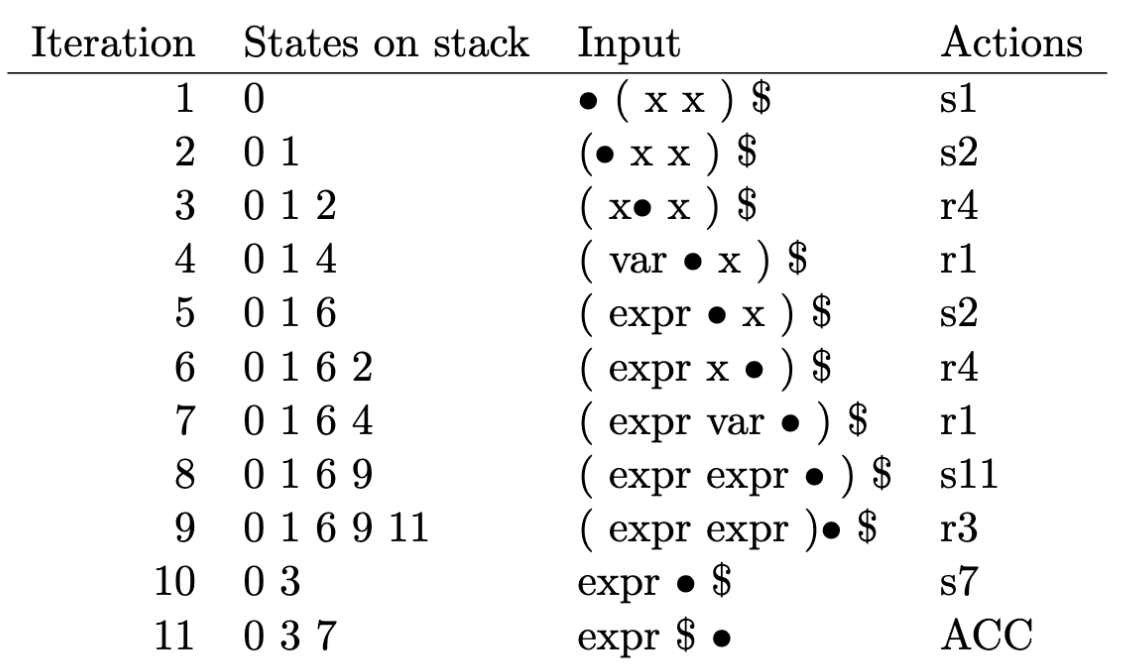
\includegraphics[width=0.5\columnwidth]{./img/lambda0.png}
  \end{figure}
    \item $(\lambda x . x)$
    \begin{figure}[htbp]
    \centering
    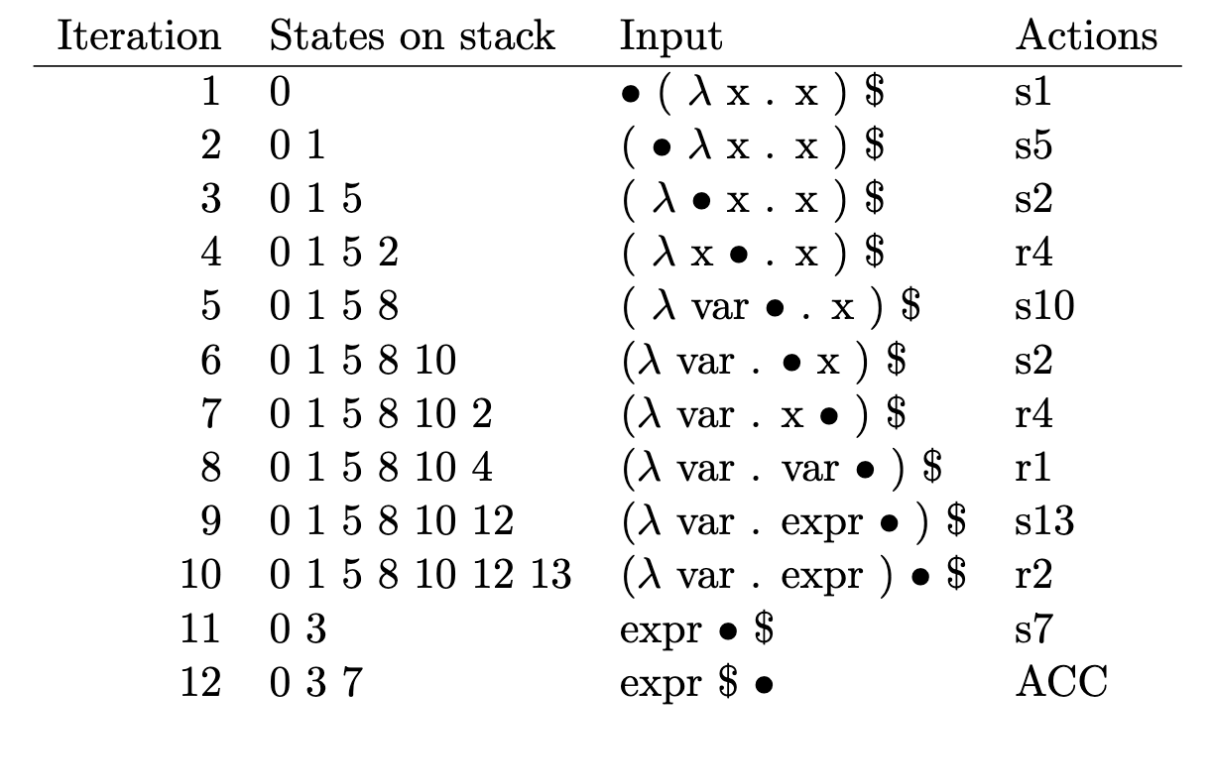
\includegraphics[width=0.5\columnwidth]{./img/lambda1.png}
  \end{figure}
  \item $(x(\lambda x . x))$
   \begin{figure}[htbp]
    \centering
    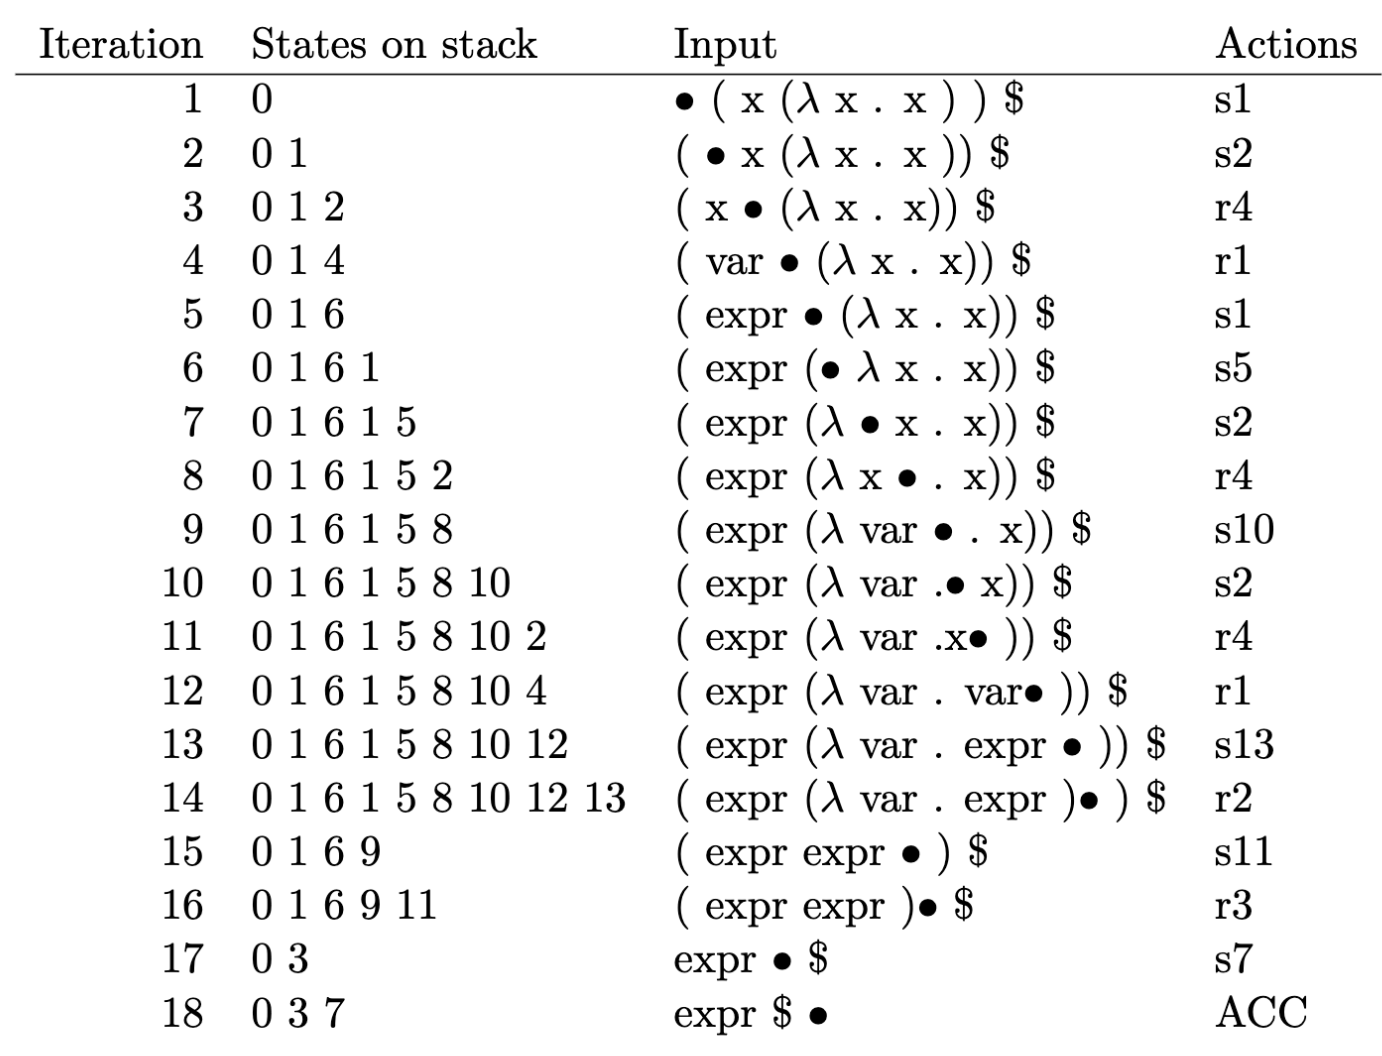
\includegraphics[width=0.5\columnwidth]{./img/lambda2.png}
  \end{figure}
\end{enumerate}


\subsubsection{Altering the Lambda Calculus.}
Suppose we want to add an optional extension that allows raising avarto a power.We define the grammar as
\begin{alltt}
  expr : var 
       | var '-' NUM
       | ‘(’ ‘\(\lambda\)’ var ‘.’ expr ‘)’
       | ‘(’ expr expr ‘)’ ;
  var  : ID ;
  \end{alltt}
  \begin{enumerate}
    \item Is this grammar LR(0)?
    \item Which state in the parsing table would we need to modify to parse this grammar?
  \end{enumerate}

\begin{solution}
\begin{enumerate}
    \item No, we don't know whether to reduce 'var' until we check for '\^'. It is LR(1).
    \item We would need to add an extra case for shifting on the lookahead symbol '\^' in State 4.
\end{enumerate}
\end{solution}


\subsection{Stack in Shift-Reduce Parsing.}
Suppose  it  is  given  that  shift-reduce  parsing  is  equivalent  to  finding  the  right most derivation in reverse.  Prove that during shift-reduce parsing, we can only reduce the top most items in the stack (i.e.  we don’t need to worry about reducing something in the middle; hence the usage of a stack is justified)

The idea of $L R(0)$ Parsing is (Assume current State $I$, next input symbol $a$ ):
\begin{enumerate}
    \item If $X \rightarrow \alpha_{1}, \in I$, Reduce by $X \rightarrow \alpha_{1}$
    \item If $X \rightarrow \alpha_{2} \cdot a \beta \in I$, Shift with $a$
    \item Considers no Token Look-aheads, so called 0
\end{enumerate}
A Configuration is $\left(I_{0} X_{1} I_{1} \ldots X_{m} I_{m}, a_{i} a_{i+1} \ldots a_{n} \$\right)$, where:
\begin{enumerate}
    \item $I_{0} X_{1} I_{1} \ldots X_{m} I_{m}$ is current Stack content, bottom to top $a_{i} a_{i+1} \ldots a_{n} \$$ is the \item rest of the input Token stream
    \item Represents:
    \begin{enumerate}
        \item A snapshot at some time in the Parsing process
\item A Right-most Derivation $S \Rightarrow^{*} X_{1} \ldots X_{m} a_{i} a_{i+1} \ldots a_{n} \$$
    \end{enumerate}
\end{enumerate}
\subsubsection{Consider the following CFG, which has the set of terminals $T=\{\mathbf{a}, \mathbf{b}\}$}

$$\begin{aligned} S & \rightarrow X \mathbf{a} \\ X & \rightarrow \mathbf{a} \mid \mathbf{a} X \mathbf{b} \end{aligned}$$
\begin{enumerate}
\item Construct a DFA for viable prefiexes of this grammar using LR(0) items.
\item Identify a shift-reduce conflict in this grammar under the SLR(1) rules.
\item Assuming that an SLR(1) parser resolves shif-reduce confilcts by choosing to shift, show the operation of such a parser on the input string \textbf{aaba}.
\item Suppose that the production $X\rightarrow \epsilon$ is added to this grammar. Identify a reduce-reduce conflict in the resulting grammar under the SLR(1) rules.
\end{enumerate}
\begin{solution}\\
%\begin{enumerate}
\textbf{a)}\\
    \begin{equation}
        \begin{aligned}
            S' &\rightarrow .S\$ \\
            S &\rightarrow .Xa \\
            X &\rightarrow .a \\ 
            X &\rightarrow .aXb
        \end{aligned}
    \end{equation}
    Then the DFA is: \\
    \tikzset{every picture/.style={line width=0.75pt}} %set default line width to 0.75pt
    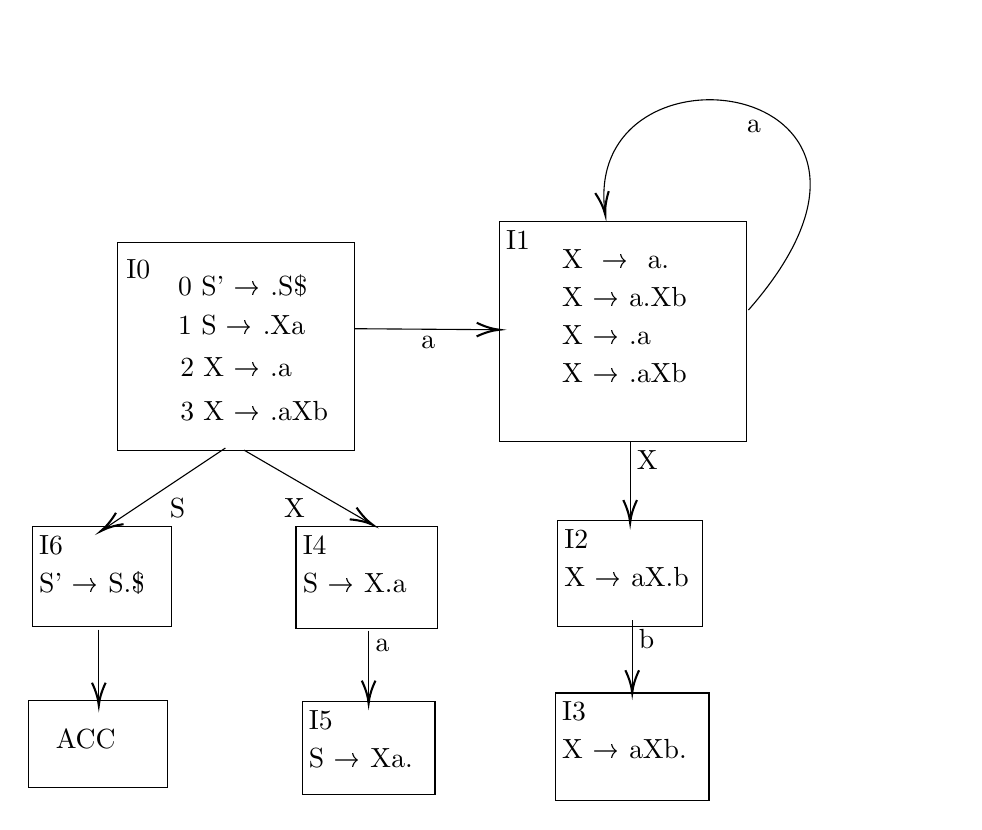
\begin{tikzpicture}[x=0.75pt,y=0.75pt,yscale=-1,xscale=1]
        %uncomment if require: \path (0,722); %set diagram left start at 0, and has height of 722
        
        %Shape: Rectangle [id:dp2132265168474865] 
        \draw   (229,219) -- (343,219) -- (343,319) -- (229,319) -- cycle ;
        %Shape: Rectangle [id:dp7940538890843964] 
        \draw   (413,209) -- (532,209) -- (532,315) -- (413,315) -- cycle ;
        %Shape: Rectangle [id:dp10282865454602796] 
        \draw   (441,353) -- (511,353) -- (511,404) -- (441,404) -- cycle ;
        %Shape: Rectangle [id:dp18723207907441308] 
        \draw   (440,436) -- (514,436) -- (514,488) -- (440,488) -- cycle ;
        %Shape: Rectangle [id:dp3836855361443223] 
        \draw   (315,356) -- (383,356) -- (383,405) -- (315,405) -- cycle ;
        %Shape: Rectangle [id:dp2664223170575777] 
        \draw   (318,440) -- (382,440) -- (382,485) -- (318,485) -- cycle ;
        %Shape: Rectangle [id:dp35626870944716416] 
        \draw   (188,356) -- (255,356) -- (255,404) -- (188,404) -- cycle ;
        %Straight Lines [id:da3538077000003601] 
        \draw    (343,260.5) -- (411,260.99) ;
        \draw [shift={(413,261)}, rotate = 180.41] [color={rgb, 255:red, 0; green, 0; blue, 0 }  ][line width=0.75]    (10.93,-3.29) .. controls (6.95,-1.4) and (3.31,-0.3) .. (0,0) .. controls (3.31,0.3) and (6.95,1.4) .. (10.93,3.29)   ;
        %Straight Lines [id:da17424455977368303] 
        \draw    (290,319) -- (350.27,354) ;
        \draw [shift={(352,355)}, rotate = 210.14] [color={rgb, 255:red, 0; green, 0; blue, 0 }  ][line width=0.75]    (10.93,-3.29) .. controls (6.95,-1.4) and (3.31,-0.3) .. (0,0) .. controls (3.31,0.3) and (6.95,1.4) .. (10.93,3.29)   ;
        %Straight Lines [id:da5447309272722132] 
        \draw    (281,318) -- (222.66,356.89) ;
        \draw [shift={(221,358)}, rotate = 326.31] [color={rgb, 255:red, 0; green, 0; blue, 0 }  ][line width=0.75]    (10.93,-3.29) .. controls (6.95,-1.4) and (3.31,-0.3) .. (0,0) .. controls (3.31,0.3) and (6.95,1.4) .. (10.93,3.29)   ;
        %Straight Lines [id:da6537981145388738] 
        \draw    (350,406) -- (350,439) ;
        \draw [shift={(350,441)}, rotate = 270] [color={rgb, 255:red, 0; green, 0; blue, 0 }  ][line width=0.75]    (10.93,-3.29) .. controls (6.95,-1.4) and (3.31,-0.3) .. (0,0) .. controls (3.31,0.3) and (6.95,1.4) .. (10.93,3.29)   ;
        %Straight Lines [id:da1831058618871224] 
        \draw    (476,315) -- (476,352) ;
        \draw [shift={(476,354)}, rotate = 270] [color={rgb, 255:red, 0; green, 0; blue, 0 }  ][line width=0.75]    (10.93,-3.29) .. controls (6.95,-1.4) and (3.31,-0.3) .. (0,0) .. controls (3.31,0.3) and (6.95,1.4) .. (10.93,3.29)   ;
        %Straight Lines [id:da4196045548767082] 
        \draw    (477,401) -- (477,434) ;
        \draw [shift={(477,436)}, rotate = 270] [color={rgb, 255:red, 0; green, 0; blue, 0 }  ][line width=0.75]    (10.93,-3.29) .. controls (6.95,-1.4) and (3.31,-0.3) .. (0,0) .. controls (3.31,0.3) and (6.95,1.4) .. (10.93,3.29)   ;
        %Curve Lines [id:da30926966581269366] 
        \draw    (533,251.5) .. controls (631.51,139.06) and (452.8,115.73) .. (463.82,204.16) ;
        \draw [shift={(464,205.5)}, rotate = 261.78] [color={rgb, 255:red, 0; green, 0; blue, 0 }  ][line width=0.75]    (10.93,-3.29) .. controls (6.95,-1.4) and (3.31,-0.3) .. (0,0) .. controls (3.31,0.3) and (6.95,1.4) .. (10.93,3.29)   ;
        %Shape: Rectangle [id:dp44819130358800785] 
        \draw   (186,439.5) -- (253,439.5) -- (253,481.5) -- (186,481.5) -- cycle ;
        %Straight Lines [id:da048082389033083706] 
        \draw    (220,405.5) -- (220,440) ;
        \draw [shift={(220,442)}, rotate = 270] [color={rgb, 255:red, 0; green, 0; blue, 0 }  ][line width=0.75]    (10.93,-3.29) .. controls (6.95,-1.4) and (3.31,-0.3) .. (0,0) .. controls (3.31,0.3) and (6.95,1.4) .. (10.93,3.29)   ;
        
        % Text Node
        \draw (232,226) node [anchor=north west][inner sep=0.75pt]   [align=left] {I0};
        % Text Node
        \draw (257,233) node [anchor=north west][inner sep=0.75pt]   [align=left] {0 S' → .S$\displaystyle \$\ \ $};
        % Text Node
        \draw (257,253) node [anchor=north west][inner sep=0.75pt]   [align=left] {1 S → .Xa$ $};
        % Text Node
        \draw (258,273) node [anchor=north west][inner sep=0.75pt]   [align=left] {2 X → .a};
        % Text Node
        \draw (258,294) node [anchor=north west][inner sep=0.75pt]   [align=left] {3 X → .aXb};
        % Text Node
        \draw (415,212) node [anchor=north west][inner sep=0.75pt]   [align=left] {I1};
        % Text Node
        \draw (442,221) node [anchor=north west][inner sep=0.75pt]   [align=left] {X \ → \ a.\\X → a.Xb\\X → .a \\X → .aXb};
        % Text Node
        \draw (443,356) node [anchor=north west][inner sep=0.75pt]   [align=left] {I2 \\X → aX.b};
        % Text Node
        \draw (442,439) node [anchor=north west][inner sep=0.75pt]   [align=left] {I3 \\X → aXb.};
        % Text Node
        \draw (317,359) node [anchor=north west][inner sep=0.75pt]   [align=left] {I4 \\S → X.a};
        % Text Node
        \draw (320,443) node [anchor=north west][inner sep=0.75pt]   [align=left] {I5\\S → Xa.};
        % Text Node
        \draw (190,359) node [anchor=north west][inner sep=0.75pt]   [align=left] {I6\\S' → S.\$};
        % Text Node
        \draw (374,263) node [anchor=north west][inner sep=0.75pt]   [align=left] {a};
        % Text Node
        \draw (531,159) node [anchor=north west][inner sep=0.75pt]   [align=left] {a};
        % Text Node
        \draw (253,341) node [anchor=north west][inner sep=0.75pt]   [align=left] {S};
        % Text Node
        \draw (308,341) node [anchor=north west][inner sep=0.75pt]   [align=left] {X};
        % Text Node
        \draw (352,409) node [anchor=north west][inner sep=0.75pt]   [align=left] {a};
        % Text Node
        \draw (478,318) node [anchor=north west][inner sep=0.75pt]   [align=left] {X};
        % Text Node
        \draw (479,404) node [anchor=north west][inner sep=0.75pt]   [align=left] {b};
        % Text Node
        \draw (198,452.5) node [anchor=north west][inner sep=0.75pt]   [align=left] {ACC};
    \end{tikzpicture}
\\ 
\textbf{b)} 
    Identify a shift-reduce conflict in this grammar under the SLR(1) rules.
    \begin{table}[H]
        \begin{tabular}{l|lll|ll}
        \hline
          & a     & b  & \$  & S & X \\ \hline
        0 & s1    &    &     & 6 & 4 \\
        1 & s1,r2 &    &     &   & 2 \\
        2 &       & s3 &     &   &   \\
        3 & r3    &    & r3  &   &   \\
        4 & s5    &    &     &   &   \\
        5 & r2    &    & r2  &   &   \\
        6 &       &    & acc &   &  
        \end{tabular}
    \end{table}
    \\
\textbf{c)} Shift-reduce parsing
    \begin{table}[H]
        \begin{tabular}{llll}
        stack  & Input  & Action                     & Output               \\
        0      & aaba\$ & shift1                     &                      \\
        0a1    & aba\$  & shift 1                    &                      \\
        0a1a1  & ba\$   & reduce X-\textgreater{}a   & X -\textgreater a    \\
        0a1X2  & ba\$   & shift 3                    &                      \\
        0a1X2b & a\$    & reduce X-\textgreater{}aXb & X -\textgreater aXb  \\
        0X3    & a\$    & shift 1                    &                      \\
        0X3a1  & \$     & reduce S -\textgreater Xa  & S -\textgreater Xa   \\
        0S6    & \$     & reduce S' -\textgreater S  & S' -\textgreater S\$ \\
        0S'    & \$     & Accept                     &                     
        \end{tabular}
    \end{table}
\textbf{d)} In the state $I_{3}$, both operations reduce $a$ to $X$ or applying $X \rightarrow \epsilon$ is OK.
%\end{enumerate}
\end{solution}

\subsection{Consider the following CFG, draw the LR(0) Autometa}
$$E\rightarrow E+T$$
$$E\rightarrow T$$
$$T\rightarrow TF$$
$$T\rightarrow F$$
$$F\rightarrow *$$
$$F\rightarrow a$$
$$F\rightarrow b$$
\begin{solution}
SLR => First(非终结符的第一个字符)/Follow(紧跟在非终结符后的第一个字符)/LR(0)项目集。详见\href{程序猿说}{https://www.bilibili.com/video/BV1Xx41187Y4}
\end{solution}
\section{More on Syntax-directed Translation}
The set of all finite strings over the alphabet $\{0,1\}$ that generate all the binary number including digits (e.g. 110.0110).

\begin{enumerate}
    \item Write the syntax-directed translation scheme (SDT) with S-attributed definition.
\begin{solution}
\begin{equation}
    \begin{aligned}
    S &\rightarrow A,B\{S.val = A.val+B.val\}\\
    S  &\rightarrow A\{S.val = A.val\} \\
    A  &\rightarrow A_{1}digit\{A.val = A_{1}.val*2+digit.val\} \\
    A  &\rightarrow digit\{A.val = digit.val\} \\
    B  &\rightarrow digit B_{1}\{B.val = B_{1}.val/2+digit.val/2\} \\
    B  &\rightarrow digit\{B.val = digit.val/2\} \\
    digit  &\rightarrow 0\{digit.val=0\}\\
    digit  &\rightarrow 1s\{digit.val=1\}
    \end{aligned}
\end{equation}
\end{solution}
\item Write the syntax-directed translation scheme (SDT) with L-attributed definition.
\begin{solution}
\begin{equation}
    \begin{aligned}
    S  &\rightarrow \{A.in=0\}A.B\{S.syn=A.syn+B.syn\} \\
    S  &\rightarrow \{A.in=0\}A\{S.syn=A.syn\} \\
    A  &\rightarrow digit\{A_{1}.in=A.in*2+digit.val\}A_{1}\{A.syn=A_{1}.syn\} \\
    A  &\rightarrow digit\{A.syn=A.in*2+digit.val\} \\
    B  &\rightarrow digit B_{1}\{B.syn=B_{1}.syn/2+digit.val/2\} \\
    B  &\rightarrow digit\{B.syn=digit.val/2\} \\
    digit  &\rightarrow 0\{digit.val=0\}\\
    digit  &\rightarrow 1\{digit.val=1\}
    \end{aligned}
\end{equation}
\end{solution}
\item Using the CFG you wrote, provide a derivation for the following input string: $10.1011$
\begin{solution}
Using SDT with S-attributed definition in (i), the right-most derivation is:
\begin{equation}
    \begin{aligned}
    S &\rightarrow A.B\{S.val=A.val+B.val\} \\
    \\
    &\rightarrow A.digit_{1}B_{1}\{B.val=B_{1}.val/2+digit_{1}.val/2\}\{S.val=A.val+B.val\} \\ 
    \\
    &\rightarrow A.digit_{1}digit_{2}B_{2}\{B_{1}.val=B_{2}.val/2+digit_{2}.val/2\}\{B.val=B_{1}.val/2+digit_{1}.val/2\}\\ &\{S.val=A.val+B.val\} \\
    \\
    &\rightarrow A.digit_{1}digit_{2}digit_{3}B_{3}\{B_{2}.val = B_{2}.val/2+digit_{3}.val/2\}\{B_{1}.val=B_{2}.val/2+digit_{2}.val/2\}\\ &\{B.val=B_{1}.val/2+digit_{1}.val/2\}\{S.val = A.val+B.val\}\\
    \\
    &\rightarrow A.digit_{1}digit_{2}digit_{3}digit_{4}\{B_{4}.val=digit_{4}.val/2\}\{B_{2}.val=B_{2}.val/2+digit_{3}.val/2\}\\ &\{B_{1}.val=B_{2}.val/2+digit.val/2\}\{B.val=B_{1}.val/2+digit_{1}.val/2\}\\ &\{B.val=B_{1}.val/2+digit_{1}.val/2\}\{S.val=A.val+B.val\} \\
    \\
    &\rightarrow A_{1}digit_{5}\{A.val=A_{1}.val*2+digit_{5}.val\}.digit_{1}digit_{2}digit_{3}digit_{4}\{B_{3}.val=digit_{4}.val/2\}\\ &\{B_{2}.val=B_{2}.val/2+digit_{3}.val/2\}\{B_{1}.val=B_{2}.val/2+digit_{2}.val/2\}\\ 
    &\{B.val=B_{1}.val/2+digit_{1}.val/2\}\{S.val=A.val+B.val\}\\
    \\
    &\rightarrow digit_{6}\{A_{1}.val=digit_{6}.val\}digit_{5}\{A.val=A_{1}.val*2+digit_{5}.val\}.digit_{1}digit_{2}digit_{3}digit_{4}\\ &\{B_{3}.val=digit_{4}.val/2\}\{B_{2}.val=B_{2}.val/2+digit_{3}.val/2\}\{B_{1}.val=B_{2}.val/2+digit_{2}.val/2\}\\ 
    &\{B.val=B_{1}.val/2+digit_{1}.val/2\}\{S.val=A.val+B.val\} 
    \end{aligned}
\end{equation}
\end{solution}
\end{enumerate}
\end{document}
